% LuaLaTeX

\documentclass[a4paper, twoside, 12pt]{article}
\usepackage[latin]{babel}
%\usepackage[landscape, left=3cm, right=1.5cm, top=2cm, bottom=1cm]{geometry} % okraje stranky
%\usepackage[landscape, a4paper, mag=1166, truedimen, left=2cm, right=1.5cm, top=1.6cm, bottom=0.95cm]{geometry} % okraje stranky
\usepackage[landscape, a4paper, mag=1400, truedimen, left=0.5cm, right=0.5cm, top=0.5cm, bottom=0.5cm]{geometry} % okraje stranky

\usepackage{fontspec}
\setmainfont[FeatureFile={junicode.fea}, Ligatures={Common, TeX}, RawFeature=+fixi]{Junicode}
%\setmainfont{Junicode}

% shortcut for Junicode without ligatures (for the Czech texts)
\newfontfamily\nlfont[FeatureFile={junicode.fea}, Ligatures={Common, TeX}, RawFeature=+fixi]{Junicode}

\usepackage{multicol}
\usepackage{color}
\usepackage{lettrine}
\usepackage{fancyhdr}

% usual packages loading:
\usepackage{luatextra}
\usepackage{graphicx} % support the \includegraphics command and options
\usepackage{gregoriotex} % for gregorio score inclusion
\usepackage{gregoriosyms}
\usepackage{wrapfig} % figures wrapped by the text
\usepackage{parcolumns}
\usepackage[contents={},opacity=1,scale=1,color=black]{background}
\usepackage{tikzpagenodes}
\usepackage{calc}
\usepackage{longtable}
\usetikzlibrary{calc}

\setlength{\headheight}{14.5pt}

% Commands used to produce a typical "Conventus" booklet

\newenvironment{titulusOfficii}{\begin{center}}{\end{center}}
\newcommand{\dies}[1]{#1

}
\newcommand{\nomenFesti}[1]{\textbf{\Large #1}

}
\newcommand{\celebratio}[1]{#1

}

\newcommand{\hora}[1]{%
\vspace{0.5cm}{\large \textbf{#1}}

\fancyhead[LE]{\thepage\ / #1}
\fancyhead[RO]{#1 / \thepage}
\addcontentsline{toc}{subsection}{#1}
}

% larger unit than a hora
\newcommand{\divisio}[1]{%
\begin{center}
{\Large \textsc{#1}}
\end{center}
\fancyhead[CO,CE]{#1}
\addcontentsline{toc}{section}{#1}
}

% a part of a hora, larger than pars
\newcommand{\subhora}[1]{
\begin{center}
{\large \textit{#1}}
\end{center}
%\fancyhead[CO,CE]{#1}
\addcontentsline{toc}{subsubsection}{#1}
}

% rubricated inline text
\newcommand{\rubricatum}[1]{\textit{#1}}

% standalone rubric
\newcommand{\rubrica}[1]{\vspace{3mm}\rubricatum{#1}}

\newcommand{\notitia}[1]{\textcolor{red}{#1}}

\newcommand{\scriptura}[1]{\hfill \small\textit{#1}}

\newcommand{\translatioCantus}[1]{\vspace{1mm}%
{\noindent\footnotesize \nlfont{#1}}}

% pruznejsi varianta nasledujiciho - umoznuje nastavit sirku sloupce
% s prekladem
\newcommand{\psalmusEtTranslatioB}[3]{
  \vspace{0.5cm}
  \begin{parcolumns}[colwidths={2=#3}, nofirstindent=true]{2}
    \colchunk{
      \input{#1}
    }

    \colchunk{
      \vspace{-0.5cm}
      {\footnotesize \nlfont
        \input{#2}
      }
    }
  \end{parcolumns}
}

\newcommand{\psalmusEtTranslatio}[2]{
  \psalmusEtTranslatioB{#1}{#2}{8.5cm}
}


\newcommand{\canticumMagnificatEtTranslatio}[1]{
  \psalmusEtTranslatioB{#1}{temporalia/extra-adventum-vespers/magnificat-boh.tex}{12cm}
}
\newcommand{\canticumBenedictusEtTranslatio}[1]{
  \psalmusEtTranslatioB{#1}{temporalia/extra-adventum-laudes/benedictus-boh.tex}{10.5cm}
}

% volne misto nad antifonami, kam si zpevaci dokresli neumy
\newcommand{\hicSuntNeumae}{\vspace{0.5cm}}

% prepinani mista mezi notovymi osnovami: pro neumovane a neneumovane zpevy
\newcommand{\cantusCumNeumis}{
  \setgrefactor{17}
  \global\advance\grespaceabovelines by 5mm%
}
\newcommand{\cantusSineNeumas}{
  \setgrefactor{17}
  \global\advance\grespaceabovelines by -5mm%
}

% znaky k umisteni nad inicialu zpevu
\newcommand{\superInitialam}[1]{\gresetfirstlineaboveinitial{\small {\textbf{#1}}}{\small {\textbf{#1}}}}

% pars officii, i.e. "oratio", ...
\newcommand{\pars}[1]{\textbf{#1}}

\newenvironment{psalmus}{
  \setlength{\parindent}{0pt}
  \setlength{\parskip}{5pt}
}{
  \setlength{\parindent}{10pt}
  \setlength{\parskip}{10pt}
}

%%%% Prejmenovat na latinske:
\newcommand{\nadpisZalmu}[1]{
  \hspace{2cm}\textbf{#1}\vspace{2mm}%
  \nopagebreak%

}

% mode, score, translation
\newcommand{\antiphona}[3]{%
\hicSuntNeumae
\superInitialam{#1}
\includescore{#2}

#3
}
 % Often used macros
%%%% Preklady jednotlivych zpevu (nektere se opakuji, a je dobre mit je
% vsechny na jedne hromade)

\newcommand{\trOratioAnteOfficium}{\translatioCantus{Otevři, Pane, má ústa, abych chválil tvé svaté jméno.
Očisti mé srdce od všech marnivých, zvrácených a~jiných myšlenek, osvěť rozum, rozněť cit,
abych mohl důstojně, soustředěně a~zbožně recitovat a~vysloužil si být
vyslyšen před tváří tvé velebnosti. Skrze Krista…}}

\newcommand{\trOratioPostOfficium}{\translatioCantus{\textit{Následující modlitbu
opatřil pro ty, kdo ji zbožně vyřknou po hodinkách, zesnulý papež Lev X.
odpustky za hříchy vzniklé při konání hodinek z~lidské křehkosti. Říká se
vkleče.}
Svatosvaté a~nerozdílné Trojici, ukřižovanému lidství našeho Pána Ježíše
Krista, přeblažené a~přeslavné plodné neporušenosti vždy Panny Marie
i~souhrnu všech svatých buď ode všeho stvoření věčná chvála, čest a~sláva, nám
pak buď dáno odpuštění všech hříchů, po nekonečné věky věků. Amen.}}

% HOURS ---

\newcommand{\trAntI}{\translatioCantus{Jasné narození slavné Panny Marie,
z pokolení (dosl. ze semene) Abrahámova, vzešlé z kmene Judova, z rodu Davidova.}}
\newcommand{\trAntII}{\translatioCantus{Dnes je Narození svaté Panny 
Marie, jejíž předrahý život osvěcuje všechny církve.}}

\newcommand{\trAntIII}{\translatioCantus{Maria, jež vzešla 
z královského rodu, září; myslí i duchem ji zbožně prosíme, aby 
nám pomáhala svými přímluvami.}}

\newcommand{\trAntIV}{\translatioCantus{Srdcem i duchem pějme Kristu 
k slávě o této svaté slavnosti vznešené Rodičky Boží Marie.}}

\newcommand{\trAntV}{\translatioCantus{Příjemně \notitia{?} 
oslavujme Narození blahoslavené Marie,
aby se ona za nás přimlouvala u Pána Ježíše Krista.}}

\newcommand{\trCapituli}{\translatioCantus{Před věky, na počátku mě stvořil, potrvám věčně. Ve svatém Stanu jsem před ním konala službu.}}

\newcommand{\trRespVesp}{\translatioCantus{Buď zdráva, Maria,
plná milosti: \grestar{} Pán s tebou. \Vbardot{} Požehnaná jsi mezi ženami,
a požehnaný plod života (ve smyslu lůna, břicha) tvého.}}

\newcommand{\trVersus}{\translatioCantus{\Vbardot{} Dnes je Narození svaté Panny Marie. \Rbardot{} Jejíž předrahý život osvěcuje všechny církve.}}

\newcommand{\trAntMagnificatI}{\translatioCantus{Konejme památku
veledůstojného narození slavné Panny Marie,
jíž se dostalo mateřské důstojnosti bez ztráty panenské cudnosti.}}

% Tento preklad je vice nez nejisty a ani alternativy, ktere jsem
% videl, me nepresvedcily...
\newcommand{\trAntBenedictus}{\translatioCantus{Slavnostně slavme 
dnešní narození Marie, vždy Panny a Rodičky Boží: v něm se objevuje
vysokost trůnu (totiž Marie, trůnu Božího Syna), aleluja.}}

\newcommand{\trAntMagnificatII}{\translatioCantus{Tvé narození,
Bohorodičko Panno, vyhlásilo radost celému světu:
z tebe totiž vzešlo Slunce spravedlnosti, Kristus, náš Bůh:
jenž zrušil kletbu a dal nám požehnání: přemohl smrt a dal nám život věčný.}}

\newcommand{\trOrationis}{\translatioCantus{Prosíme tě, Bože, 
uděl svým služebníkům dar nebeské milosti,
aby těm, jimž slehnutím blahoslavené Panny vyvstal počátek spásy, 
slavnost k poctě jejího narození přinesla
rozhojnění pokoje.
Skrze tvého Syna, našeho Pána Ježíše Krista, který s tebou žije a kraluje,
Bůh, v jednotě Ducha svatého po všechny věky věků.}}

\newcommand{\trFideliumAnimae}{\translatioCantus{\Vbardot{} Duše věrných ať pro
milosrdenství Boží odpočívají v~pokoji. \Rbardot{} Amen.}}

% Completorium

\newcommand{\trJubeDomne}{\translatioCantus{Rač, pane, požehnat.}}

\newcommand{\trComplBenedictio}{\translatioCantus{Pokojnou noc a~svatou smrt
nechť nám dopřeje všemohoucí Pán. \Rbardot{} Amen.}}

\newcommand{\trComplLectioBr}{\translatioCantus{Buďte střízliví, bděte.
Váš protivník Ďábel obchází jako lev řvoucí a~hledá, koho by pohltil.
Postavte se proti němu pevní ve víře.  Ale ty, Pane, smiluj se nad námi.
\Rbardot{} Bohu díky.}}

\newcommand{\trComplAntI}{\translatioCantus{Rač se smilovati nade mnou,
Hospodine, a vyslyš mou modlitbu.}}

\newcommand{\trComplCapituli}{\translatioCantus{Jsi přece, Hospodine,
uprostřed nás a~jmenujeme se po tobě.  Neopouštěj nás, Pane, náš Bože.}}

\newcommand{\trRespCompl}{\translatioCantus{Do tvých rukou, Pane, \grestar{}
poroučím svého ducha. \Vbardot{} Ty mne zachráníš, Pane, Bože věrný.}}

\newcommand{\trComplVersus}{\translatioCantus{\Vbardot{} Střez mne jako zřítelnici oka,
aleluja. \Rbardot{} Ve stínu svých křídel uschovej mne, aleluja.}}

\newcommand{\trAntSalvaNos}{\translatioCantus{Ochraňuj nás, Pane, když
bdíme, a~buď s~námi, když spíme, ať bdíme s~Kristem a~odpočíváme v~pokoji.}}

\newcommand{\trComplOrationis}{\translatioCantus{Zavítej, prosíme, Pane, sem
do našeho příbytku a~daleko od něj zažeň všechny úklady nepřítele. Ať tu
bydlí tví svatí andělé a~tvoje požehnání buď nad ním stále. Skrze…}}

\newcommand{\trSalveRegina}{\translatioCantus{Zdrávas Královno, matko
milosrdenství, živote, sladkosti a naděje naše, buď zdráva!
K tobě voláme, vyhnaní synové Evy,
k tobě vzdycháme, lkajíce a plačíce
v tomto slzavém údolí.
A proto, orodovnice naše,
obrať k nám své milosrdné oči
a Ježíše, požehnaný plod života svého,
nám po tomto putování ukaž,
ó milostivá, ó přívětivá,
ó přesladká, Panno Maria!}}

\newcommand{\trOraProNobis}{\translatioCantus{\Vbardot{} 
Oroduj za nás, svatá Boží Rodičko,
\Rbardot{} aby nám Kristus dal účast na svých zaslíbeních.}}

% Matutinum

\newcommand{\trMatInvitatorium}{\translatioCantus{}}

\newcommand{\trMatVeniteA}{\translatioCantus{Pojďte, chvalme s~radostí Pána,
s~jásotem slavme Boha, svou spásu; předstupme před tvář jeho s~díky, písně plesu pějme jemu.}}

\newcommand{\trMatVeniteB}{\translatioCantus{Neboť Bůh veliký jest Hospodin, a~král nade všecky bohy.
Jsouť v~jeho ruce všecky hlubiny země, temena hor jsou majetek jeho.}}

\newcommand{\trMatVeniteC}{\translatioCantus{Jehoť jest moře, neb on je učinil; i~souš
je dílo jeho rukou. Pojďme, klanějme se, padněme, klekněme před Pánem, svým
tvůrcem. Jeť on Pán, náš Bůh, a~my jsme lid, jejž on vodí a~ovce, jež pase.}}

\newcommand{\trMatVeniteD}{\translatioCantus{Kéž byste poslechli dnes hlasu jeho:
,,Nezatvrzujte svých srdcí jak v~Hádce, jak v~Pokušení na poušti, kde vaši otcové pokoušeli mne,
zkoušeli mne, ač vídali skutky mé.``}}

\newcommand{\trMatVeniteE}{\translatioCantus{Čtyřicet roků mrzel jsem se na to pokolení
a~řekl jsem: ,,Lid je to myslí stále bloudící``! Oni však nechtěli znáti mé cesty, takže jsem
přisáhl ve svém hněvu: ,,Nedojdou odpočinku mého!\mbox{}``}}

\newcommand{\trMatAntI}{\translatioCantus{}}

\newcommand{\trMatAntII}{\translatioCantus{}}

\newcommand{\trMatAntIII}{\translatioCantus{}}

\newcommand{\trMatVersusI}{\translatioCantus{}}

\newcommand{\trMatAbsolutioI}{\translatioCantus{Vyslyš Pane Ježíši Kriste
prosby svých služebníků \gredagger{} a~smiluj se nad námi, \grestar{} jenž
s~Otcem a~Duchem…}}

\newcommand{\trMatBenedictioI}{\translatioCantus{Rač, pane, požehnat.
Věčný Otec nám stále žehnej. \Rbardot{} Amen.}}

\newcommand{\trMatLecI}{\translatioCantus{Kéž by mě zulíbal polibky svých úst. 
Tvé milování je nad víno lahodnější;
vybraně voní tvé voňavky;
rozlévající se olej je tvé jméno,
proto tě dívky milují.
Strhni mě za sebou, poběžme!
Král mě uvedl do svých komnat;
budeš nám radostí a jásotem.
Víc než víno oslavíme tvé milování;
věru po právu jsi milován!
Snědá jsem, a přece krásná, jeruzalémské dcery,
jako stany kedarské,
jako šalmské závěsy.
}}

\newcommand{\trMatRespI}{\translatioCantus{}}

\newcommand{\trMatBenedictioII}{\translatioCantus{Rač, pane, požehnat.
Jednorozený Boží Syn nám žehnej \grestar{} a nám pomáhej. \Rbardot{} Amen.}}

\newcommand{\trMatLecII}{\translatioCantus{Nehleďte na mou osmahlou pleť:
to mě slunce ožehlo.
Synové mé matky se na mne rozzlobili,
poslali mě hlídat vinice.
A svou vinici, tu jsem nehlídala!
Pověz mi tedy, ty, jehož miluje mé srdce:
kam zavedeš své stádo pást,
kde ho necháš za poledne odpočívat?
Abych už nebloudila jako tulačka
poblíž stád druhů tvých.
Nevíš-li to, nejrásnější z žen,
jdi po stopách stáda
a kůzlata svá zaveď, ať se pasou
poblíž obydlí pastýřů.
Ke své klisně zapřažené do vozu faraonova
tebe, mé milá, přirovnávám.
Stále krásné jsou tvé líce s náušnicemi
i tvé hrdlo v náhrdelnících.}}

\newcommand{\trMatRespII}{\translatioCantus{}}

\newcommand{\trMatBenedictioIII}{\translatioCantus{Rač, pane, požehnat.
Milost Ducha Svatého ať osvítí nám smysly \grestar{} i srdce. \Rbardot{} Amen.}}

\newcommand{\trMatLecIII}{\translatioCantus{Zhotovíme ti zlaté náušnice
a kuličky ze stříbra.
Když král stoluje,
vydechuje můj nard svou vůni.
Můj milý je polštářek s myrhou,
jenž mi odpočívá mezi ňadry.
Můj milý je hrozen šáchoru
ve vinicích v Engadi.
Jak jsi krásná, milá moje,
jak jsi krásná!
Tvé oči jsou holubice.
Jak jsi krásný, můj milý,
jak líbezný!
Naše lože je samá zeleň.
Trámoví našeho domu je z cedru,
naše ostění z cypřiše.}}

\newcommand{\trMatRespIII}{\translatioCantus{}}

\newcommand{\trMatAntIV}{\translatioCantus{}}

\newcommand{\trMatAntV}{\translatioCantus{}}

\newcommand{\trMatAntVI}{\translatioCantus{}}

\newcommand{\trMatVersusII}{\translatioCantus{}}

\newcommand{\trMatAbsolutioII}{\translatioCantus{
Tvá milost a laskavost nechť nám pomáhá, jenž žiješ a vládneš s Otcem a Svatým Duchem na věky věků.}}

\newcommand{\trMatBenedictioIV}{\translatioCantus{Rač, pane, požehnat.
Bůh Otec všemohoucí, \grestar{} buď k nám milostivý a odpouštějící. \Rbardot{} Amen.}}

\newcommand{\trMatLecIV}{\translatioCantus{}}

\newcommand{\trMatRespIV}{\translatioCantus{}}

\newcommand{\trMatBenedictioV}{\translatioCantus{}}

\newcommand{\trMatLecV}{\translatioCantus{}}

\newcommand{\trMatRespV}{\translatioCantus{}}

\newcommand{\trMatBenedictioVI}{\translatioCantus{Rač, pane, požehnat.
Bůh rozněť v nás oheň své lásky. \Rbardot{} Amen.}}

\newcommand{\trMatLecVI}{\translatioCantus{}}

\newcommand{\trMatRespVI}{\translatioCantus{}}

\newcommand{\trMatAntVII}{\translatioCantus{}}

\newcommand{\trMatAntVIII}{\translatioCantus{}}

\newcommand{\trMatAntIX}{\translatioCantus{}}

\newcommand{\trMatVersusIII}{\translatioCantus{}}

\newcommand{\trMatAbsolutioIII}{\translatioCantus{Z okovů našich hříchů,
\grestar{} vysvoboď nás všemohoucí a milosrdný Pán. \Rbardot{} Amen.}}

\newcommand{\trMatBenedictioVII}{\translatioCantus{Rač, pane, požehnat.
Čtení evangelia nechť je nám \grestar{} spásou a ochranou. \Rbardot{} Amen.}}

\newcommand{\trMatLecVIIa}{\translatioCantus{
  Rodokmen Ježíše Krista, syna Davidova, syna Abrahámova:
  Abrahám zplodil Izáka,
  Izák zplodil Jakuba.}}

\newcommand{\trMatLecVIIb}{\translatioCantus{}}

\newcommand{\trMatRespVII}{\translatioCantus{}}

\newcommand{\trMatBenedictioVIII}{\translatioCantus{Rač, pane, požehnat.
\Rbardot{} Amen.}}

\newcommand{\trMatLecVIII}{\translatioCantus{}}

\newcommand{\trMatRespVIII}{\translatioCantus{}}

\newcommand{\trMatBenedictioIX}{\translatioCantus{Rač, pane, požehnat.
Do společnosti občanů nebes \grestar{} ať nás dovede král andělů.
\Rbardot{} Amen.}}

\newcommand{\trMatLecIX}{\translatioCantus{}}

% from the Czech Liturgia horarum
\newcommand{\trTeDeum}{\begin{translatioMulticol}{3}

Bože, tebe chválíme, 
tebe, Pane, velebíme.

Tebe, věčný Otče, 
oslavuje celá země.

Všichni andělé, 
cherubové i~serafové,

všechny mocné nebeské zástupy 
bez ustání volají:

Svatý, Svatý, Svatý, 
Pán, Bůh zástupů.

Plná jsou nebesa i~země 
tvé vznešené slávy.

Oslavuje tě 
sbor tvých apoštolů,

chválí tě 
velký počet proroků,

vydává o~tobě svědectví 
zástup mučedníků;

a~po celém světě 
vyznává tě tvá církev:

neskonale velebný, 
všemohoucí Otče,

úctyhodný Synu Boží, 
pravý a~jediný,

božský Utěšiteli, 
Duchu svatý.

Kriste, Králi slávy, 
tys od věků Syn Boha Otce;

abys člověka vykoupil, 
stal ses člověkem a~narodil ses z~Panny;

zlomil jsi osten smrti 
a~otevřel věřícím nebe;

sedíš po Otcově pravici 
a~máš účast na jeho slávě.

Věříme, že přijdeš soudit, 

a~proto tě prosíme:
přispěj na pomoc svým služebníkům, 
vždyť jsi je vykoupil svou předrahou krví;

dej, ať se radují s~tvými svatými 
ve věčné slávě.

Zachraň, Pane, svůj lid, žehnej svému dědictví, 
veď ho a~stále pozvedej.

Každý den tě budeme velebit 
a~chválit tvé jméno po všechny věky.

Pomáhej nám i~dnes, 
ať se nedostaneme do područí hříchu.

Smiluj se nad námi, Pane, 
smiluj se nad námi.

Ať spočine na nás tvé milosrdenství, 
jak doufáme v~tebe.

Pane, k~tobě se utíkáme, 
ať nejsme zahanbeni na věky. 
\end{translatioMulticol}}

\newcommand{\trMatEvangelium}{\translatioCantus{
  Rodokmen Ježíše Krista, syna Davidova, syna Abrahámova:
  Abrahám zplodil Izáka,
  Izák zplodil Jakuba,
  Jakub zplodil Judu a jeho bratry,
  Juda zplodil Farese a Zaru z Tamary,
  Fares zplodil Esroma,
  Esrom zplodil Arama,
  Aram zplodil Aminadaba,
  Aminadab zplodil Naasona,
  Naason zplodil Salmona,
  Salmon zplodil Boaze z Rahaby,
  Boaz zplodil Jobeda z Rut,
  Jobed zplodil Jessea,
  Jesse zplodil krále Davida.
  David zplodil Šalomouna z Uriášovy ženy,
  Šalomoun zplodil Roboama,
  Roboam zplodil Abiu,
  Abia zplodil Asu,
  Asa zplodil Josafata,
  Josafat zplodil Jorama,
  Joram zplodil Oziáše,
  Oziáš zplodil Joatama,
  Joatam zplodil Achaze,
  Achaz zplodil Ezechiáše,
  Ezechiáš zplodil Manasesa,
  Manases zplodil Amona,
  Amon zplodil Josiáše,
  Josiáš zplodil Jechoniáše a jeho bratry;
  tehdy došlo k odvlečení do Babylonu.
  Po odvlečení do Babylonu:
  Jechoniáš zplodil Salatiela,
  Salatiel zplodil Zorobabela,
  Zorobabel zplodil Abiuda,
  Abiud zplodil Eljakima,
  Eljakim zplodil Azora,
  Ator zplodil Sadoka,
  Sadok zplodil Achima,
  Achim zplodil Eliuda,
  Eliud zplodil Eleazara,
  Eleatar zplodil Matana,
  Matan zplodil Jakuba,
  Jakub zplodil Josefa, manžela Marie,
  z níž se narodil Ježíš, který se nazývá Kristus.}}

\newcommand{\trTeDecetLaus}{\translatioCantus{Tobě chvála, Tobě zpěvy, Tobě
sláva, Bohu Otci i~Synu i~Svatému Duchu, na věky věků. \Rbardot{} Amen.}}

% MASS ---

\newcommand{\trIntroitus}{\translatioCantus{Radujme se všichni
v Pánu, slavíce svátek ke cti Panny Marie: z něj se radují andělé
a spoluchválí Božího Syna. \textit{\color{red}Žl.} Má ústa vydala dobré slovo,
přednáším svá díla králi.}}

\newcommand{\trGraduale}{\translatioCantus{Požehnaná a ctihodná jsi,
Panno Maria: nedotčená (co do panenství) jsi byla shledána matkou
Spasitele. \Vbardot{} Panno Boží Rodičko, ten, jehož nepojme ani celý svět,
se uzavřel do tvých útrob, když se stal člověkem.}}

\newcommand{\trAlleluia}{\translatioCantus{Aleluja. \Vbardot{} Skvělá slavnost
slavné Panny Marie, z pokolení (dosl. ze semene) Abrahámova, vzešlé z kmene 
Judova, z rodu Davidova.}}

\newcommand{\trOffertorium}{\translatioCantus{Blažená jsi, Panno Maria,
tys nosila Stvořitele všeho; porodila jsi toho, který tě utvořil,
a na věky zůstáváš Pannou.}}

\newcommand{\trCommunio}{\translatioCantus{Budou mě blahoslavit
všechna pokolení, protože mi učinil veliké věci ten, který je mocný.}}

% LITTLE HOURS ---

\newcommand{\trVersusTertia}{\translatioCantus{\Vbardot{} \Rbardot{}}}

\newcommand{\trCapituliEtSic}{\translatioCantus{
Tak jsem se usadila na Sionu a v milovaném městě jsem nalezla odpočinek,
v Jeruzalémě vykonávám svou moc.
Zakořenila jsem u lidu plného slývy, na panství Páně, v jeho dědictví.}}

\newcommand{\trVersusSexta}{\translatioCantus{\Vbardot{} \Rbardot{}}}

\newcommand{\trCapituliInPlateis}{\translatioCantus{
Na planině jako skořicovník a akant jsem vydávala vůni, jako vybraná myrha
jsem voněla.}}

\newcommand{\trVersusNona}{\translatioCantus{\Vbardot{} \Rbardot{}}}
 % Czech translations of the proper texts

\newcommand{\annusEditionis}{2020}

%%%% Vicekrat opakovane kousky

\newcommand{\anteOrationem}{
  \rubrica{Ante Orationem, cantatur a Superiore:}

  \pars{Supplicatio Litaniæ.}

  \cuminitiali{}{temporalia/supplicatiolitaniae.gtex}

  \pars{Oratio Dominica.}

  \cuminitiali{}{temporalia/oratiodominica.gtex}

  \rubrica{Deinde dicitur ab Hebdomadario:}

  \cuminitiali{}{temporalia/dominusvobiscum-solemnis.gtex}

  \rubrica{In choro monialium loco Dominus vobiscum dicitur:}

  \sineinitiali{temporalia/domineexaudi.gtex}
}

\setlength{\columnsep}{30pt} % prostor mezi sloupci

%%%%%%%%%%%%%%%%%%%%%%%%%%%%%%%%%%%%%%%%%%%%%%%%%%%%%%%%%%%%%%%%%%%%%%%%%%%%%%%%%%%%%%%%%%%%%%%%%%%%%%%%%%%%%
\begin{document}

% Here we set the space around the initial.
% Please report to http://home.gna.org/gregorio/gregoriotex/details for more details and options
\grechangedim{afterinitialshift}{2.2mm}{scalable}
\grechangedim{beforeinitialshift}{2.2mm}{scalable}
\grechangedim{interwordspacetext}{0.22 cm plus 0.15 cm minus 0.05 cm}{scalable}%
\grechangedim{annotationraise}{-0.2cm}{scalable}

% Here we set the initial font. Change 38 if you want a bigger initial.
% Emit the initials in red.
\grechangestyle{initial}{\color{red}\fontsize{38}{38}\selectfont}

\pagestyle{empty}

%%%% Titulni stranka
\begin{titulusOfficii}
\dies{Dominica ultima per annum.}
\nomenFesti{In Festo Domini Nostri Iesu Christi Universorum Regis.}
\celebratio{Duplex I. classis.}
\end{titulusOfficii}

% graphic
%\vspace{1.5cm}
%\begin{center}
%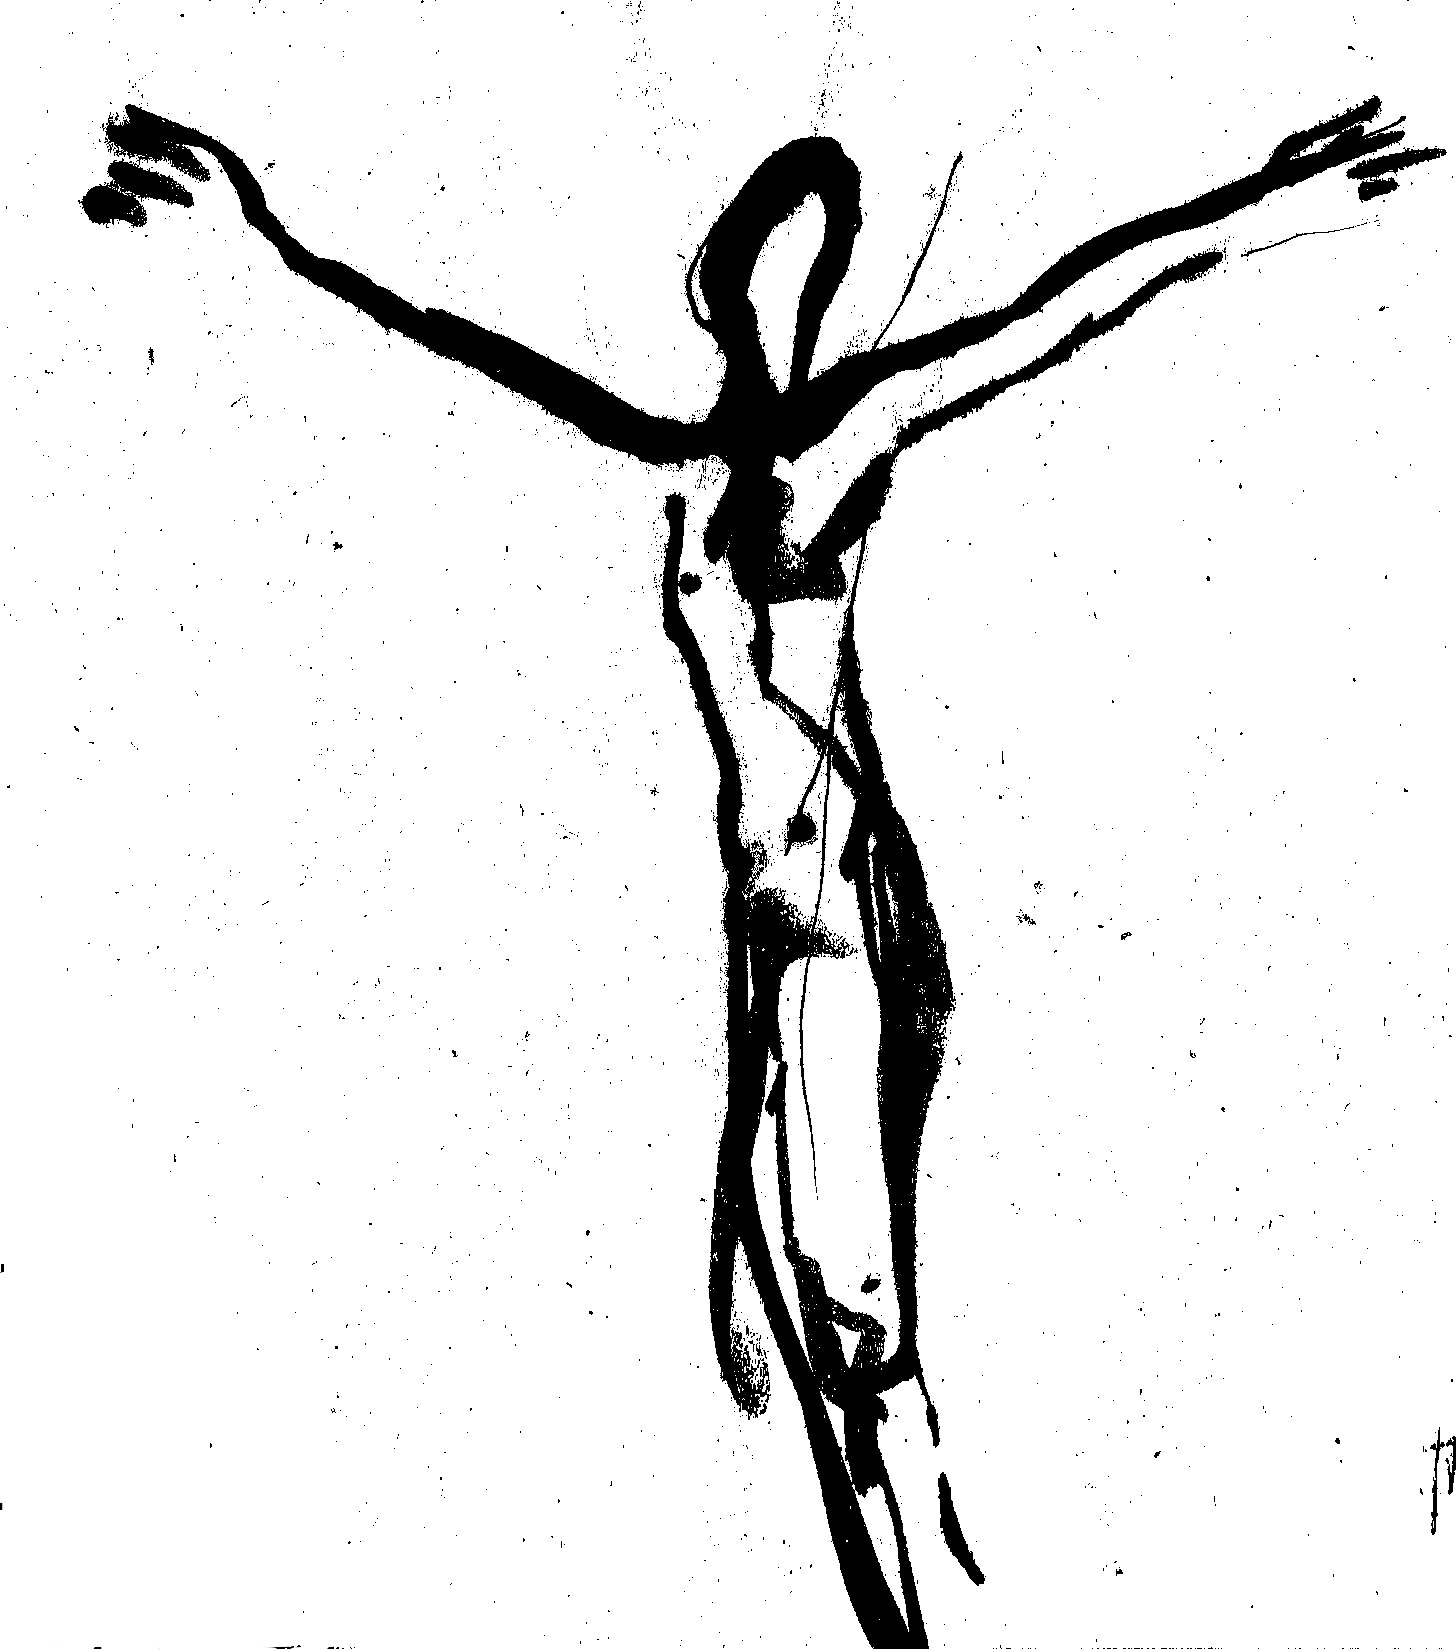
\includegraphics[height=8cm]{crux.jpg}
%\end{center}

\vfill

\begin{center}
%Ad usum et secundum consuetudines chori \guillemotright{}Conventus Choralis\guillemotleft.

%Editio Sancti Wolfgangi \annusEditionis
\end{center}

\pagebreak

\renewcommand{\headrulewidth}{0pt} % no horiz. rule at the header
\fancyhf{}
\pagestyle{fancy}

\cantusSineNeumas

\pars{Oratio ante divinum Officium.}

\lettrine{{\color{red}A}}{peri,} Dómine, os meum ad benedicéndum nomen sanctum tuum:
munda quoque cor meum ab ómnibus vanis, pervérsis, et aliénis
cogitatiónibus:
intelléctum illúmina, afféctum inflámma,
ut digne, atténte ac devóte hoc Offícium recitáre váleam,
et exaudíri mérear ante conspéctum Divínæ Maiestátis tuæ.
Per Christum, Dóminum nostrum.
\Rbardot{} Amen.

Dómine, in unióne illíus divínæ intentiónis,
qua ipse in terris laudes Deo persolvísti,
has tibi Horas \rubricatum{(vel \textnormal{hanc tibi Horam})} persólvo.

%\trOratioAnteOfficium

\vfill

\pars{Oratio post divinum Officium.}

\rubrica{
  Orationem sequentem devote post Officium recitantibus
  Leo Papa X. defectus, et culpas in eo persolvendo ex humana
  fragilitate contractas, indulsit, et dicitur flexis genibus.
}

\lettrine{{\color{red}S}}{acrosánctæ} et indivíduæ Trinitáti,
crucifíxi Dómini nostri Iesu Christi humanitáti,
beatíssimæ et gloriosíssimæ sempérque Vírginis Maríæ
fecúndæ integritáti, 
et ómnium Sanctórum universitáti
sit sempitérna laus, honor, virtus et glória
ab omni creatúra,
nobísque remíssio ómnium peccatórum,
per infiníta sǽcula sæculórum.
\Rbardot{} Amen.

\noindent \Vbardot{} Beáta víscera Maríæ Virginis, quæ portavérunt
ætérni Patris Fílium.\\
\Rbardot{} Et beáta úbera, quæ lactavérunt Christum Dominum.

\rubrica{Et dicitur secreto \textnormal{Pater noster.} et \textnormal{Ave María.}}

%\trOratioPostOfficium

\vfill

\pars{} \scriptura{}

\hora{Ad I. Vesperas.} %%%%%%%%%%%%%%%%%%%%%%%%%%%%%%%%%%%%%%%%%%%%%%%%%%%%%
%\sideThumbs{I. Vesperæ}

\vspace{5mm}
\grechangedim{interwordspacetext}{0.18 cm plus 0.15 cm minus 0.05 cm}{scalable}%
\cuminitiali{}{temporalia/deusinadiutorium-solemnis.gtex}
\grechangedim{interwordspacetext}{0.22 cm plus 0.15 cm minus 0.05 cm}{scalable}%

\vfill
\pagebreak

\pars{Psalmus 1.} \scriptura{1 Par. 22, 9; 17, 14}

\vspace{-4mm}

\antiphona{VIII G}{temporalia/ant-pacificusvocabitur.gtex}

%\trAntI

\scriptura{Ps. 112}

\initiumpsalmi{temporalia/ps112-initium-viii-G-auto.gtex}

%\psalmusEtTranslatioT{temporalia/ps112-comb.tex}{10cm}
\input{temporalia/ps112.tex} \Abardot{}

\vfill
\pagebreak

\pars{Psalmus 2.} \scriptura{Dan. 7, 27}

\vspace{-4mm}

\antiphona{VIII c\textsuperscript{2}}{temporalia/ant-regnumeius.gtex}

%\trAntII

\scriptura{Ps. 116}

\initiumpsalmi{temporalia/ps116-initium-viii-C2-auto.gtex}
%\psalmusEtTranslatioT{temporalia/ps116-comb.tex}{10cm}
\input{temporalia/ps116.tex} \Abardot{}

\vfill
\pagebreak

\pars{Psalmus 3.} \scriptura{Zach. 6, 12.13; 9, 10}

\vspace{-4mm}

\antiphona{VII c\textsuperscript{2}}{temporalia/ant-ecceviroriens.gtex}

%\trAntIII

\scriptura{Ps. 144, 1-9}

\initiumpsalmi{temporalia/ps144i-initium-vii-c2-auto.gtex}
%\psalmusEtTranslatioT{temporalia/ps144i-comb.tex}{10cm}
\input{temporalia/ps144i.tex} \Abardot{}

\vfill
\pagebreak

\pars{Psalmus 4.} \scriptura{Cf. Dan. 7, 14; \textbf{H78}}

\vspace{-4mm}

\antiphona{VIII G}{temporalia/ant-christodatusest.gtex}

%\trAntIV

%\vspace{-2mm}

\scriptura{Ps. 144, 10-21}

%\vspace{-2mm}

\initiumpsalmi{temporalia/ps144ii-initium-viii-G-auto.gtex}
%\psalmusEtTranslatioT{temporalia/ps144ii-comb.tex}{10cm}
\input{temporalia/ps144ii.tex} \Abardot{}

\vfill
\pagebreak

% Capitulum. %%%
\pars{Capitulum.} \scriptura{1 Cor. 15, 25-28}

\cuminitiali{}{temporalia/capitulum-OportetChristus.gtex}

% preklad Jeruz. bible
%\trCapituli

\vfill
\pars{Responsorium.} \scriptura{\Rbardot{} 1 Paral. 29, 11 \Vbardot{} 2 Mac. 1, 24; \textbf{H424}}

\vspace{-5mm}

\responsorium{II}{temporalia/resp-tuaestpotentia-CROCHU-cumdox.gtex}{}

%\trRespVesp

\vfill
\pagebreak

% Hymnus. %%%
\pars{Hymnus.}

{
\grechangedim{interwordspacetext}{0.20 cm plus 0.15 cm minus 0.05 cm}{scalable}%
\cuminitiali{I}{temporalia/hym-TeSaeculorum.gtex}
\grechangedim{interwordspacetext}{0.22 cm plus 0.15 cm minus 0.05 cm}{scalable}%
}
%\input{cantus/amon33/hym-TeSaeculorum-bohtext.tex}

\vfill

\pars{Versus.} \scriptura{Mt. 28, 17}

% Versus. %%%
\sineinitiali{temporalia/versus-dataest.gtex}
    
\noindent %\trVersus

\vfill
\pagebreak

\pars{Canticum B. Mariæ V.} \scriptura{Cf. Lc. 1, 51.52; \textbf{H424}}

\vspace{-4mm}

\antiphona{VII b}{temporalia/ant-magnificemus.gtex}

%\trAntMagnificatI

%\vspace{-3mm}

\scriptura{Lc. 1, 46-55}

\vspace{-2mm}

\initiumpsalmi{temporalia/magnificat-initium-viisoll-b.gtex}

%\vspace{-1.5mm}

%\psalmusEtTranslatioT{temporalia/magnificat-comb.tex}{10.3cm}
\input{temporalia/magnificat.tex} \Abardot{}

\vfill
\pagebreak

\anteOrationem

\pagebreak

%% Oratio. %%%
\pars{Oratio.}

\cuminitiali{}{temporalia/oratio.gtex}
%\trOrationis

\vfill

\rubrica{Hebdomadarius dicit iterum Dominus vobiscum, vel cantor dicit:}

\vspace{2mm}

\sineinitiali{temporalia/domineexaudi.gtex}

\rubrica{Postea cantatur a cantore:}

\vspace{2mm}

\cuminitiali{II}{temporalia/benedicamus-solemnism-1vesp.gtex}

\vspace{1mm}

\vfill
\pagebreak

\iffalse
\hora{Ad Matutinum.} %%%%%%%%%%%%%%%%%%%%%%%%%%%%%%%%%%%%%%%%%%%%%%%%%%%%%%%%%%
%\sideThumbs{Matutinum}

\vspace{2mm}

\cantusSineNeumas

\cuminitiali{}{temporalia/dominelabiamea.gtex}

\vspace{5mm}

\pars{Invitatorium.} \scriptura{Cantor; \textbf{K183r}}

\vspace{-2mm}

\antiphona{II}{temporalia/inv-regemregum.gtex}

\vfill
\pagebreak

\pars{Hymnus.}

\vspace{-5mm}

\antiphona{I}{temporalia/hym-ChristeCaelorum.gtex}

\vfill
\pagebreak

\subhora{In I. Nocturno}

\pars{Psalmus 1.} \scriptura{Ps. 1, 2.6; \textbf{H331}}

\vspace{-4mm}

\antiphona{VIII G\textsuperscript{3}}{temporalia/ant-novitdominus.gtex}

%\trMatAntI

\scriptura{Psalmus 1.}

\initiumpsalmi{temporalia/ps1-initium-viii-G3.gtex}

%\psalmusEtTranslatioT{temporalia/ps1-comb.tex}{10cm}
\input{temporalia/ps1.tex} \Abardot{}

\vfill
\pagebreak

\pars{Psalmus 2.} \scriptura{Ps. 4, 4; \textbf{H331}}

\vspace{-4mm}

\antiphona{VII c\textsuperscript{2}}{temporalia/ant-mirificavit.gtex}

%\trMatAntII

\scriptura{Psalmus 4.}

\initiumpsalmi{temporalia/ps4-initium-vii-c2-auto.gtex}

%\psalmusEtTranslatioT{temporalia/ps4-comb.tex}{10cm}
\input{temporalia/ps4.tex} \Abardot{}

\vfill
\pagebreak

\pars{Psalmus 3.} \scriptura{Ps. 8, 2; \textbf{H331}}

\vspace{-4mm}

\antiphona{I D\textsuperscript{2}}{temporalia/ant-admirabileest.gtex}

%\trMatAntIII

\scriptura{Psalmus 8.}

\initiumpsalmi{temporalia/ps8-initium-i-D2-auto.gtex}

%\psalmusEtTranslatioT{temporalia/ps8-comb.tex}{10cm}
\input{temporalia/ps8.tex} \Abardot{}

\vfill
\pagebreak

\pars{Versus.} \scriptura{Ps. 31, 11}

\sineinitiali{temporalia/versus-laetamini-communis.gtex}

\vspace{5mm}

\sineinitiali{temporalia/oratiodominica-mat.gtex}

\vspace{5mm}

\pars{Absolutio.}

\cuminitiali{}{temporalia/absolutio-exaudi.gtex}

%\trMatAbsolutioI

\vfill
\pagebreak

\cuminitiali{}{temporalia/benedictio-solemn-benedictione.gtex}

%\trMatBenedictioI

\vspace{7mm}

\pars{Lectio I.} \scriptura{Ap. 1, 4-6}

\noindent De libro Apocalýpsis beáti Ioánnis Apóstoli.

\noindent Grátia vobis et pax ab eo qui est et qui erat et qui ventúrus est, et a septem spirítibus qui in conspéctu throni eius sunt, et a Iesu Christo, qui est testis fidélis, primogénitus mortuórum et princeps regum terræ, qui diléxit nos et lavit nos a peccátis nostris in sánguine suo, et fecit nos regnum et sacerdótes Deo et Patri suo: ipsi glória et impérium in sǽcula sæculórum. Amen.

\noindent \Vbardot{} Tu autem, Dómine, miserére nobis.
\noindent \Rbardot{} Deo grátias.

\vfill
\pagebreak

\pars{Responsorium 1.} \scriptura{\Rbardot{} Esth. 13, 9 \Vbardot{} ibid. 13, 17; \textbf{H411}}

\vspace{-5mm}

\responsorium{II}{temporalia/resp-dominerexomnipotens-CROCHU.gtex}{}

\vfill
\pagebreak

\cuminitiali{}{temporalia/benedictio-solemn-unigenitus.gtex}

%\trMatBenedictioII

\vspace{7mm}

\pars{Lectio II.} \scriptura{Ap. 1, 10.12-18}

\noindent Fui in spíritu in domínica die, et audívi post me vocem magnam tamquam tubæ. Et convérsus sum ut vidérem vocem quæ loquebátur mecum; et convérsus vidi septem candelábra áurea, et in médio septem candelabrórum aureórum símilem fílio hóminis vestítum podére et præcínctum ad mamíllas zona áurea. Caput autem eius et capílli erant cándidi tamquam lana alba et tamquam nix, et óculi eius tamquam flamma ignis, et pedes eius símiles aurichálco, sicut in camíno ardénti, et vox illíus tamquam vox aquárum multárum. Et habébat in déxtera sua stellas septem, et de ore eius gládius utráque parte acútus exíbat, et fácies eius sicut sol lucet in virtúte sua. Et cum vidíssem eum, cécidi ad pedes eius tamquam mórtuus; et pósuit déxteram suam super me, dicens: ,,Noli timére; ego sum primus et novíssimus, et vivus et fui mórtuus, et ecce sum vivens in sǽcula sæculórum; et hábeo claves mortis et inférni.``

\noindent \Vbardot{} Tu autem, Dómine, miserére nobis.
\noindent \Rbardot{} Deo grátias.

\vfill
\pagebreak

\pars{Responsorium 2.} \scriptura{\Rbardot{} Is. 6, 1 \Vbardot{} Is. 6, 2; \textbf{H416}}

\vspace{-5mm}

\responsorium{I}{temporalia/resp-vididominumsedentem-CROCHU-sinedox.gtex}{}

\vfill
\pagebreak

\cuminitiali{}{temporalia/benedictio-solemn-spiritus.gtex}

%\trMatBenedictioIII

\vspace{7mm}

\pars{Lectio III.} \scriptura{Ap. 2, 26.28; 3, 5.12.20-21}

\noindent ,,Qui vícerit et custodíerit usque in finem ópera mea, dabo illi potestátem super gentes, sicut et ego accépi a Patre meo; et dabo illi stellam matutínam. Et non delébo nomen eius de libro vitæ, et confitébor nomen eius coram Patre meo et coram ángelis eius. Fáciam illum colúmnam in templo Dei mei, et foras non egrediétur ámplius; et scribam super eum nomen Dei mei et nomen civitátis Dei mei, novæ Ierúsalem, quæ descéndit de cælo a Deo meo, et nomen meum novum. Ecce sto ad óstium et pulso; si quis audíerit vocem meam et aperúerit mihi iánuam, intrábo ad illum et cenábo cum illo, et ipse mecum. Qui vícerit, dabo ei sedére mecum in throno meo, sicut et ego vici et sedi cum Patre meo in throno eius.``

\noindent \Vbardot{} Tu autem, Dómine, miserére nobis.
\noindent \Rbardot{} Deo grátias.

\vfill
\pagebreak

\pars{Responsorium 3.} \scriptura{\Rbardot{} Idt. 9, 17 \Vbardot{} ibid. 9, 16; \textbf{H410}}

\vspace{-5mm}

\responsorium{II}{temporalia/resp-dominatordomine-CROCHU-cumdox.gtex}{}}

\vfill
\pagebreak

\subhora{In II. Nocturno}

\pars{Psalmus 4.} \scriptura{Ps. 14, 1.2; \textbf{H331}}

\vspace{-4mm}

\antiphona{VI F}{temporalia/ant-dominequioperati.gtex}

%\trMatAntIV

\scriptura{Psalmus 14.}

\initiumpsalmi{temporalia/ps14-initium-vi-F-auto.gtex}

%\psalmusEtTranslatioT{temporalia/ps14-comb.tex}{10cm}
\input{temporalia/ps14.tex} \Abardot{}

\vfill
\pagebreak

\pars{Psalmus 5.} \scriptura{Ps. 23, 6; \textbf{H331}}

\vspace{-4mm}

\antiphona{III a}{temporalia/ant-haecestgeneratio.gtex}

%\trMatAntV

\scriptura{Psalmus 23.}

\initiumpsalmi{temporalia/ps23-initium-iii-a.gtex}

%\psalmusEtTranslatioT{temporalia/ps23iiia-comb.tex}{10cm}
\input{temporalia/ps23iiia.tex} \Abardot{}

\vfill
\pagebreak

\pars{Psalmus 6.} \scriptura{Ps. 31, 11; \textbf{H331}}

\vspace{-6mm}

\antiphona{VIII G}{temporalia/ant-laetamini.gtex}

%\trMatAntVI

\vspace{-2mm}

\scriptura{Psalmus 31.}

\vspace{-2mm}

\initiumpsalmi{temporalia/ps31-initium-viii-G-auto.gtex}

\vspace{-1mm}

%\psalmusEtTranslatioT{temporalia/ps31-comb.tex}{10cm}
\input{temporalia/ps31.tex} \Abardot{}

\vfill
\pagebreak

\pars{Versus.} \scriptura{Ps. 67, 4}

\sineinitiali{temporalia/versus-exsultabunt-communis.gtex}

\vspace{5mm}

\sineinitiali{temporalia/oratiodominica-mat.gtex}

\vspace{5mm}

\pars{Absolutio.}

\cuminitiali{}{temporalia/absolutio-ipsius.gtex}

%\trMatAbsolutioII

\vfill
\pagebreak

\cuminitiali{}{temporalia/benedictio-solemn-deus.gtex}

%\trMatBenedictioIV

\vspace{7mm}

\pars{Lectio IV.} \scriptura{Cap. 25: PG 11, 495-499}

\noindent Ex Libéllo Orígenis presbýteri De oratióne.

\noindent Si regnum Dei, iuxta verbum Dómini et Servatóris nostri, cum observatióne non venit, neque dicent: Ecce hic aut ecce illic; sed regnum Dei intra nos est, nam prope est verbum valde in ore nostro et in corde nostro: procul dúbio is qui regnum Dei adveníre precátur, de eo quod in se habet regno Dei recte orat, ut oriátur et fructus ferat et perficiátur. Nam in quólibet sanctórum Deus regnat et quílibet sanctus spiritálibus obséquitur légibus Dei, qui in ipso hábitat ut in recte administráta civitáte. Præsens ei Pater adest et conrégnat Patri Christus in illa ánima perfécta iuxta illud: Ad eum veniémus, et mansiónem apud eum faciémus.

\noindent \Vbardot{} Tu autem, Dómine, miserére nobis.
\noindent \Rbardot{} Deo grátias.

\vfill
\pagebreak

\pars{Responsorium 4.} \scriptura{\Rbardot{} 2 Mac. 14, 35-36 \Vbardot{} Ps. 79, 2; \textbf{H415}}

\vspace{-5mm}

\responsorium{II}{temporalia/resp-tudomineuniversorum-CROCHU.gtex}{}

\vfill
\pagebreak

\cuminitiali{}{temporalia/benedictio-solemn-christus.gtex}

%\trMatBenedictioV

\vspace{7mm}

\pars{Lectio V.}

\noindent Tunc ergo id quod in nobis est regnum Dei perpétuo procedéntibus nobis ad summum pervéniet, cum illud implétum fúerit quod Apóstolus ait, Christum subiéctis sibi ómnibus inimícis traditúrum regnum Deo et Patri, ut sit Deus ómnia in ómnibus. Propter hoc indesinénter orántes ea ánimi affectióne, quæ Verbo divína fiat, dicámus Patri nostro, qui in cælis est: Sanctificétur nomen tuum, advéniat regnum tuum. Id quoque de regno Dei percipiéndum est: sicut non est participátio iustítiæ cum iniquitáte, neque socíetas lucis ad ténebras, neque convéntio Christi ad Bélial: sic regnum Dei cum regno peccáti stare non posse.

\noindent \Vbardot{} Tu autem, Dómine, miserére nobis.
\noindent \Rbardot{} Deo grátias.

\vfill
\pagebreak

\pars{Responsorium 5.} \scriptura{\Rbardot{} Dan. 3, 55; Is. 40, 12 \Vbardot{} Ps. 79, 2; Dan. 9, 18; \textbf{H419}}

\vspace{-5mm}

\responsorium{II}{temporalia/resp-quicaelorumcontinesthronos-CROCHU-sinedox.gtex}{}

\vfill
\pagebreak

\cuminitiali{}{temporalia/benedictio-solemn-ignem.gtex}

%\trMatBenedictioVI

\vspace{7mm}

\pars{Lectio VI.}

\noindent Ergo si Deum in nobis regnáre vólumus, nullo modo regnet peccátum in nostro mortáli córpore, sed mortificémus membra nostra, quæ sunt super terram et fructificémus Spíritu; ut in nobis, quasi in spiritáli paradíso, Deus obámbulet regnétque solus in nobis cum Christo suo, qui sédeat in nobis a dextris virtútis illíus spiritális, quam optámus accípere: sedeátque donec inimíci eius omnes, qui in nobis sunt, fiant scabéllum pedum eius et evacuétur in nobis omnis principátus et potéstas et virtus. Possunt enim hæc in unoquóque nostrum fíeri et novíssima inimíca déstrui mors; ut et in nobis Christus dicat: Ubi est, mors, stímulus tuus? Ubi est, inférne, victória tua? Iam nunc ígitur corruptíbile nostrum induátur sanctitátem et incorruptiónem; et mortále, evacuáta morte, patérnam induátur immortalitátem, ut in nobis, regnánte Deo, in regeneratiónis iam resurrectionísque bonis versémur.

\noindent \Vbardot{} Tu autem, Dómine, miserére nobis.
\noindent \Rbardot{} Deo grátias.

\vfill
\pagebreak

\pars{Responsorium 6.} \scriptura{\Rbardot{} 1 Paral. 29, 11 \Vbardot{} 2 Mac. 1, 24; \textbf{H424}}

\vspace{-5mm}

\responsorium{II}{temporalia/resp-tuaestpotentia-CROCHU-cumdox.gtex}{}

\vfill
\pagebreak

\subhora{In III. Nocturno}

\pars{Psalmus 7.} \scriptura{Ps. 33, 10.16; \textbf{H332}}

\vspace{-4mm}

\antiphona{I g\textsuperscript{2}}{temporalia/ant-timetedominum.gtex}

%\vspace{-4mm}

%\trMatAntVII

\scriptura{Psalmus 33.}

\initiumpsalmi{temporalia/ps33-initium-i-g2.gtex}

%\psalmusEtTranslatioT{temporalia/ps33-comb.tex}{10.5cm}
\input{temporalia/ps33.tex}

\vfill

\antiphona{}{temporalia/ant-timetedominum.gtex} % repeat the antiphon - new page

\vfill
\pagebreak

\pars{Psalmus 8.} \scriptura{Ps. 60, 4.5.6; \textbf{H332}}

\antiphona{III a}{temporalia/ant-dominespessanctorum.gtex}

%\trMatAntVIII

\scriptura{Psalmus 60.}

\initiumpsalmi{temporalia/ps60-initium-iii-a.gtex}

%\psalmusEtTranslatioT{temporalia/ps60iiia-comb.tex}{10cm}
\input{temporalia/ps60iiia.tex} \Abardot{}

\vfill
\pagebreak

\pars{Psalmus 9.} \scriptura{Ps. 96, 10.12; \textbf{H332}}

\antiphona{I D\textsuperscript{3}}{temporalia/ant-quidiligitis.gtex}

%\trMatAntIX

\scriptura{Psalmus 96.}

\initiumpsalmi{temporalia/ps96-initium-i-D3.gtex}

%\psalmusEtTranslatioT{temporalia/ps96-comb.tex}{10cm}
\input{temporalia/ps96.tex} \Abardot{}

\vfill
\pagebreak

\pars{Versus.} \scriptura{Sap. 5, 16}

\sineinitiali{temporalia/versus-justi.gtex}

\vspace{5mm}

\sineinitiali{temporalia/oratiodominica-mat.gtex}

\vspace{5mm}

\pars{Absolutio.}

\cuminitiali{}{temporalia/absolutio-avinculis.gtex}

%\trMatAbsolutioIII

\vfill
\pagebreak

\cuminitiali{}{temporalia/benedictio-solemn-evangelica.gtex}

%\trMatBenedictioVII

\vspace{7mm}

\pars{Lectio VII.} \scriptura{Io. 18, 33-37}

\noindent Léctio sancti Evangélii secúndum Ioánnem.

\noindent In illo témpore: Dixit Pilátus ad Iesum: Tu es Rex Iudæórum? Respóndit Iesus: A temetípso hoc dicis, an álii dixérunt tibi de me? Et réliqua.

\scriptura{CCL 3A, 97-98}

\noindent Ex Tractátu sancti Cypriáni epíscopi et mártyris De domínica oratióne.

\noindent Advéniat regnum tuum. Regnum étiam Dei repræsentári nobis pétimus, sícuti et nomen eius ut in nobis sanctificétur postulámus. Nam Deus quando non regnat, aut apud eum quando íncipit quod et semper fuit et esse non désinit? Nostrum regnum pétimus adveníre a Deo nobis repromíssum, Christi sánguine et passióne quæsítum, ut qui in sǽculo ante servívimus, póstmodum Christo dominánte regnémus, sicut ipse pollicétur et dicit: Veníte, benedícti patris mei, percípite regnum quod vobis parátum est ab orígine mundi.

\noindent \Vbardot{} Tu autem, Dómine, miserére nobis.
\noindent \Rbardot{} Deo grátias.

\vfill
\pagebreak

\pars{Responsorium 7.} \scriptura{\Rbardot{} Ier. 31, 11.12 \Vbardot{} Ps. 4, 8; \textbf{H418}}

\vspace{-5mm}

\responsorium{III}{temporalia/resp-redemitdominus-CROCHU.gtex}{}

\vfill
\pagebreak

\cuminitiali{}{temporalia/benedictio-solemn-divinum.gtex}

%\trMatBenedictioVIII

\vspace{7mm}

\pars{Lectio VIII.}

\noindent Potest vero, fratres dilectíssimi, et ipse Christus esse regnum Dei quem veníre cotídie cúpimus, cuius advéntus ut cito nobis repræsentétur optámus. Nam cum resurréctio ipse sit, quia in ipso resúrgimus, sic et regnum Dei potest ipse intéllegi, quia in illo regnatúri sumus.

\noindent \Vbardot{} Tu autem, Dómine, miserére nobis.
\noindent \Rbardot{} Deo grátias.

\vfill
\pagebreak

\pars{Responsorium 8.} \scriptura{\Rbardot{} Is. 6, 3 \Vbardot{} Io. 5, 7; \textbf{Bud.\textsuperscript{118} 111v.}}

\vspace{-5mm}

\responsorium{I}{temporalia/resp-duoseraphim-cumdox.gtex}{}}

\vfill
\pagebreak

\cuminitiali{}{temporalia/benedictio-solemn-perevangelica.gtex}

%\trMatBenedictioIX

\vspace{7mm}

\pars{Lectio IX.}

\noindent Bene autem regnum Dei pétimus, id est regnum cæléste, quia est et terréstre regnum; sed qui renuntiávit iam sǽculo maior est et honóribus eius et regno. Et ídeo qui se Deo et Christo dicat non terréna sed cæléstia desíderat. Contínua autem oratióne et prece opus est, ne excidámus de regno cælésti, Dómino manifestánte et probánte: Multi, inquit, vénient ab Oriénte et Occidénte et recúmbent cum Abraham et Isaac et lacob in regno cælórum. Fílii autem regni expelléntur in ténebras exterióres: illic erit plorátio et stridor déntium. Et ídeo christiáni qui in oratióne appelláre Patrem Deum cœ́pimus, nos, et ut regnum Dei nobis véniat orámus.

\noindent \Vbardot{} Tu autem, Dómine, miserére nobis.
\noindent \Rbardot{} Deo grátias.

\vfill
\pagebreak

% Te Deum

\pars{Hymnus Ambrosianus} \scriptura{Tonus Solemnis}

\vspace{-2mm}

\grechangedim{interwordspacetext}{0.26 cm plus 0.15 cm minus 0.05 cm}{scalable}%
\cuminitiali{III}{temporalia/tedeum-solemnis-gn.gtex}
\grechangedim{interwordspacetext}{0.22 cm plus 0.15 cm minus 0.05 cm}{scalable}%

%\trTeDeum

\vfill
\pagebreak

\sineinitiali{temporalia/domineexaudi.gtex}

\vfill

\pars{Oratio.}

\cuminitiali{}{temporalia/oratio.gtex}
%\trOrationis

\vfill

\noindent \Vbardot{} Dómine, exáudi oratiónem meam.
\Rbardot{} Et clamor meus ad te véniat.

\vfill

% Nocturnale Romanum 2002, p. LXXVI Benedicamus Domino seems to match
% the one from Solemn Laudes.
\cuminitiali{V}{temporalia/benedicamus-solemnis-laud.gtex}

\vfill

\noindent \Vbardot{} Fidélium ánimæ per misericórdiam Dei requiéscant in pace.
\Rbardot{} Amen.

%\trFideliumAnimae

\vfill
\pagebreak

\hora{Ad Laudes.} %%%%%%%%%%%%%%%%%%%%%%%%%%%%%%%%%%%%%%%%%%%%%%%%%%%%%%%%%%
%\sideThumbs{Laudes}

% Psalmi festivi (AM33, pg. 721):
% 66 // 92, 99, 62, Dan3, 148+149+150

\vspace{4mm}

\cuminitiali{}{temporalia/deusinadiutorium-alter.gtex}
%\vspace{1cm}

\cantusSineNeumas

\vspace{4mm}

\pars{Psalmus 1.} \scriptura{Ap. 7, 9}

\vspace{-4mm}

\antiphona{I f}{temporalia/ant-viditurbam.gtex}

%\trAntI

\vspace{-2mm}

\scriptura{Ps. 92}

%\vspace{-2mm}

\initiumpsalmi{temporalia/ps92-initium-i-f-auto.gtex}

%\vspace{-1.5mm}

%\psalmusEtTranslatioT{temporalia/ps92-comb.tex}{10cm}
\input{temporalia/ps92.tex} \Abardot{}

\vfill
\pagebreak

\pars{Psalmus 2.} \scriptura{Ap. 7, 11}

\antiphona{I f}{temporalia/ant-etomnesangeli.gtex}

%\trAntII

\scriptura{Ps. 99}

\initiumpsalmi{temporalia/ps99-initium-i-f-auto.gtex}

%\psalmusEtTranslatioT{temporalia/ps99-comb.tex}{10cm}
\input{temporalia/ps99.tex} \Abardot{}

\vfill
\pagebreak

\pars{Psalmus 3.}

\vspace{-4mm}

\antiphona{VIII G}{temporalia/ant-redemistinos.gtex}

%\vspace{-2mm}

%\trAntIII

\scriptura{Ps. 62.}

\initiumpsalmi{temporalia/ps62-initium-viii-G-auto.gtex}

%\vspace{-6mm}

%\psalmusEtTranslatioT{temporalia/ps62-comb.tex}{10cm}
\input{temporalia/ps62.tex} \Abardot{}

\vfill
\pagebreak

\pars{Psalmus 4.} \scriptura{Dan. 3, 87}

\vspace{-4mm}

\antiphona{per.}{temporalia/ant-sanctidomini.gtex}

\vspace{-2mm}

%\trAntIV

\scriptura{Canticum trium puerorum, Dan. 3, 57-88 et 56}

\vspace{-2mm}

\initiumpsalmi{temporalia/dan3-initium-per-auto.gtex}

%\psalmusEtTranslatioT{temporalia/dan3-comb.tex}{10cm}
\input{temporalia/dan3.tex}

\rubrica{Hic non dicitur Gloria Patri, neque Amen.}
\vspace{1cm}

\antiphona{}{temporalia/ant-sanctidomini.gtex} % repeat the antiphon - new page

\vfill
\pagebreak

\pars{Psalmus 5.} \scriptura{Ps. 148, 14; Ps. 149, 9}

\vspace{-4mm}

\antiphona{VIII G}{temporalia/ant-hymnusomnibus.gtex}

\vspace{-2mm}

%\trAntV

\scriptura{Ps. 148}

\vspace{-2mm}

\initiumpsalmi{temporalia/ps148-initium-viii-G-auto.gtex}

%\vspace{-1.5mm}

%\psalmusEtTranslatioT{temporalia/ps148-comb.tex}{10cm}
\input{temporalia/ps148.tex} \rubrica{Hic non dicitur Gloria Patri.}

\vspace{-5mm}

\vfill
\pagebreak

%
\scriptura{Ps. 149}

\initiumpsalmi{temporalia/ps149-initium-viii-G-auto.gtex}

%\psalmusEtTranslatioT{temporalia/ps149-comb.tex}{10cm}
\input{temporalia/ps149.tex}

\rubrica{Hic non dicitur Gloria Patri.}

\vfill
\pagebreak

%
\scriptura{Ps. 150}

\initiumpsalmi{temporalia/ps150-initium-viii-G-auto.gtex}

%\psalmusEtTranslatioT{temporalia/ps150-comb.tex}{10cm}
\input{temporalia/ps150.tex}

\antiphona{}{temporalia/ant-hymnusomnibus.gtex} % repeat the antiphon - new page

\vfill
\pagebreak

\cantusSineNeumas

\pars{Capitulum.} \scriptura{Ap. 7, 2-3}

\cuminitiali{}{temporalia/capitulum-EcceEgo.gtex}

% preklad Jeruz. bible
%\trCapituli

\vfill
\pars{Responsorium breve.} \scriptura{Ps. 31, 11}

\antiphona{VI}{temporalia/resp-laetaminiindomino.gtex}

%\trRespVesp

\vfill
\pagebreak

% Hymnus. %%%
\pars{Hymnus.}

{
\grechangedim{interwordspacetext}{0.20 cm plus 0.15 cm minus 0.05 cm}{scalable}%
\cuminitiali{VIII}{temporalia/hym-IesuSalvator.gtex}
\grechangedim{interwordspacetext}{0.22 cm plus 0.15 cm minus 0.05 cm}{scalable}%
}
%\input{cantus/amon33/hym-TibiChriste-bohtext.tex}

\vfill

\pars{Versus.} \scriptura{Ps. 67, 4}

% Versus. %%%
\sineinitiali{temporalia/versus-exsultabunt.gtex}
    
\noindent %\trVersus

\vfill
\pagebreak

\pars{Canticum Zachariæ.} \scriptura{\textbf{H334}}

\vspace{-4mm}

\antiphona{VII a}{temporalia/ant-incivitatedomini.gtex}

%\trAntBenedictus

%\vspace{-3mm}

\scriptura{Lc. 1, 68-79}

%\vspace{-2mm}

\initiumpsalmi{temporalia/benedictus-initium-viisoll-a-auto.gtex}

%\vspace{-1.5mm}

%\psalmusEtTranslatioT{temporalia/benedictus-comb.tex}{10cm}
\input{temporalia/benedictus.tex}

\vfill

\antiphona{}{temporalia/ant-incivitatedomini.gtex}

\vfill
\pagebreak

\cantusSineNeumas

\anteOrationem

\pagebreak

% Oratio. %%%
\pars{Oratio.}

\cuminitiali{}{temporalia/oratio.gtex}
%\trOrationis

\vfill

\rubrica{Hebdomadarius dicit iterum Dominus vobiscum, vel cantor dicit:}

\vspace{2mm}

\sineinitiali{temporalia/domineexaudi.gtex}

\rubrica{Postea cantatur a cantore:}

\vspace{2mm}

\cuminitiali{II}{temporalia/benedicamus-solemnism-laud.gtex}

\vspace{1mm}

\vfill
\pagebreak

\hora{Ad II. Vesperas.} %%%%%%%%%%%%%%%%%%%%%%%%%%%%%%%%%%%%%%%%%%%%%%%%%%%%%
%\sideThumbs{II. Vesperæ}

%\vspace{5mm}
\grechangedim{interwordspacetext}{0.18 cm plus 0.15 cm minus 0.05 cm}{scalable}%
\cuminitiali{}{temporalia/deusinadiutorium-solemnis.gtex}
\grechangedim{interwordspacetext}{0.22 cm plus 0.15 cm minus 0.05 cm}{scalable}%

\vspace{4mm}

%\vfill
%\pagebreak

\pars{Psalmus 1.} \scriptura{Ap. 7, 9}

\vspace{-4mm}

\antiphona{I f}{temporalia/ant-viditurbam.gtex}

\vspace{-2mm}

%\trAntI

\scriptura{Ps. 109}

\initiumpsalmi{temporalia/ps109-initium-i-f-auto.gtex}

%\psalmusEtTranslatioT{temporalia/ps109-comb.tex}{10cm}
\input{temporalia/ps109.tex} \Abardot{}

\vfill
\pagebreak

\pars{Psalmus 2.} \scriptura{Ps. 14, 1; \textbf{H254}}

\antiphona{VII a}{temporalia/ant-incaelestibusregnis.gtex}

%\trAntII

\scriptura{Ps. 111}

\initiumpsalmi{temporalia/ps111-initium-vii-a-auto.gtex}
%\psalmusEtTranslatioT{temporalia/ps111-comb.tex}{10cm}
\input{temporalia/ps111.tex} \Abardot{}

\vfill
\pagebreak

\pars{Psalmus 3.}

\antiphona{VIII G}{temporalia/ant-deustentavitillos.gtex}

%\trAntIII

\scriptura{Ps. 112}

\initiumpsalmi{temporalia/ps112-initium-viii-G-auto.gtex}
%\psalmusEtTranslatioT{temporalia/ps112-comb.tex}{10cm}
\input{temporalia/ps112.tex} \Abardot{}

\vfill
\pagebreak

\pars{Psalmus 4.} \scriptura{Ps. 148, 14; Ps. 149, 9}

\antiphona{VIII G}{temporalia/ant-hymnusomnibus.gtex}

%\trAntIV

\scriptura{Ps. 115}

\initiumpsalmi{temporalia/ps115-initium-viii-G-auto.gtex}
%\psalmusEtTranslatioT{temporalia/ps115-comb.tex}{10cm}
\input{temporalia/ps115.tex} \Abardot{}

\vfill
\pagebreak

% Capitulum. %%%
\pars{Capitulum.} \scriptura{Ap. 7, 2-3}

\cuminitiali{}{temporalia/capitulum-EcceEgo.gtex}

% preklad Jeruz. bible
%\trCapituli

\vfill
\pars{Responsorium breve.} \scriptura{Ps. 67, 4}

\vspace{-5mm}

\responsorium{VI}{temporalia/resp-exsultentjusti.gtex}{}

%\trRespVesp

\vfill
\pagebreak

% Hymnus. %%%
\pars{Hymnus.} \scriptura{Elisagarus (\olddag{} post 837)}

{
\grechangedim{interwordspacetext}{0.20 cm plus 0.15 cm minus 0.05 cm}{scalable}%
\cuminitiali{VIII}{temporalia/hym-ChristeRedemptor.gtex}
\grechangedim{interwordspacetext}{0.22 cm plus 0.15 cm minus 0.05 cm}{scalable}%
}
%\input{cantus/amon33/hym-ChristeRedemptor-bohtext.tex}

\vfill
%\pagebreak

\pars{Versus.} \scriptura{Ps. 31, 11}

% Versus. %%%
\sineinitiali{temporalia/versus-laetamini.gtex}
    
\noindent %\trVersus

\vfill
\pagebreak

\pars{Canticum B. Mariæ V.} \scriptura{Ap. 7, 13; ibid. 14, 4; \textbf{H331}}

\vspace{-6mm}

\antiphona{VI C}{temporalia/ant-oquamgloriosum.gtex}

%\trAntMagnificatII

\vspace{-3mm}

\scriptura{Lc. 1, 46-55}

\vspace{-2mm}

\initiumpsalmi{temporalia/magnificat-initium-visoll-C.gtex}

\vspace{-1.5mm}

%\psalmusEtTranslatioT{temporalia/magnificat-comb.tex}{10.3cm}
\input{temporalia/magnificat.tex} \Abardot{}

\vfill
\pagebreak

\anteOrationem

\pagebreak

%% Oratio. %%%
\pars{Oratio.}

\cuminitiali{}{temporalia/oratio.gtex}
%\trOrationis

\vfill

\rubrica{Hebdomadarius dicit iterum Dominus vobiscum, vel cantor dicit:}

\vspace{2mm}

\sineinitiali{temporalia/domineexaudi.gtex}

\rubrica{Postea cantatur a cantore:}

\vspace{2mm}

\cuminitiali{II}{temporalia/benedicamus-solemnism-2vesp.gtex}

\vspace{1mm}

\vfill
\pagebreak
\fi

\end{document}
